
\documentclass{sig-alternate}
\conferenceinfo{GECCO}{'15, Madrid, Spain}
\usepackage{graphicx}
\usepackage{subfigure}
\usepackage{multirow}
\graphicspath{{pics/}}
\usepackage{listings}
\usepackage{amsmath}
%\usepackage[]{algorithm2e}
\begin{document}

\title{Deep Parameter Optimisation}

\numberofauthors{2} %  in this sample file, there are a *total*
% of EIGHT authors. SIX appear on the 'first-page' (for formatting
% reasons) and the remaining two appear in the \additionalauthors section.
%
\author{
% You can go ahead and credit any number of authors here,
% e.g. one 'row of three' or two rows (consisting of one row of three
% and a second row of one, two or three).
%
% The command \alignauthor (no curly braces needed) should
% precede each author name, affiliation/snail-mail address and
% e-mail address. Additionally, tag each line of
% affiliation/address with \affaddr, and tag the
% e-mail address with \email.
%
% 1st. author
\alignauthor Fan Wu, Mark Harman, Yue Jia and Jens Krinke\\
       \affaddr{CREST, UCL, London, UK}
       %\affaddr{London, UK}
       %\affaddr{London WC1E 6BT, United Kingdom}\\
       %\email{fan.wu.12@ucl.ac.uk}
% 2nd. author
\alignauthor Westley Weimer\\
       \affaddr{University of Virginia}\\
       \affaddr{USA}
}
% There's nothing stopping you putting the seventh, eighth, etc.
% author on the opening page (as the 'third row') but we ask,
% for aesthetic reasons that you place these 'additional authors'
% in the \additional authors block, viz.
% Just remember to make sure that the TOTAL number of authors
% is the number that will appear on the first page PLUS the
% number that will appear in the \additionalauthors section.

\maketitle
\begin{abstract}

%
%An efficient memory allocator can help operating system save memory and make program applications run faster. This paper introduces a deep parameter optimisation technique to improve two non-functional properties, memory consumption and execution time for general purpose memory allocators. The approach extracts deep and shallow parameters to  adaptively re-tuning a memory allocator for a given specific program.
%We report experiments that show the deep parameter optimisation competes with the shallow parameter optimisation and the default configurations. For \# real world subjects, the deep parameter optimisation saves x\% of memory and reduce y\% of execution time overall.  We also present reasons why the implicit parameters exposed by our approach are meaningful to human developer. Deep parameter optimisation is thus a promising way to improve non-functional property for memory allocators.
%

\end{abstract}

% A category with the (minimum) three required fields
\category{H.4}{Information Systems Applications}{Miscellaneous}
%A category including the fourth, optional field follows...
\category{D.2.8}{Software Engineering}{Metrics}[complexity measures, performance measures]

\terms{Theory}

\keywords{Parameter tuning, parameter exposure, dynamic memory allocator} % NOT required for Proceedings



\section{Introduction}

To achieve optimal performance, many software systems need to be configured according to workload and running environment. 
Software developers often expose a set of parameters for users to re-configure such software systems adaptively.
However, manual parameter tuning is a demanding challenge because users are usually required not only to have extensive knowledge about the system and the workload, but also to balance many competing objectives, such as memory consumption and execution time.

Many studies have reported on the challenge of automated parameter tuning \cite{Hoffmann:2011:DKR:1950365.1950390, Vuduc01statisticalmodels,autotuning,Whaley:1998:ATL:509058.509096,Tapus:2002:AHT:762761.762771, hutter2009paramils,arcuri-ssbse-2011}. Early work attempted to find optimal values with mathmatical approaches \cite{Vuduc01statisticalmodels,autotuning,Whaley:1998:ATL:509058.509096,Tapus:2002:AHT:762761.762771}, while SBSE \cite{Harman:2007:CSF:1253532.1254729} has been used in more recent research \cite{hutter2009paramils,arcuri-ssbse-2011, Hoffmann:2011:DKR:1950365.1950390} on this problem. Although these approaches can automatically re-configure a system, their improvements are limited to those achievable with the given parameters.


Many software systems contain undocumented internal variables or even expressions (those can be evaluated as concrete values) that also affect the performance of the systems. Thus, these elements could also be good candidates for automated parameter tuning. However, many of these elements are `private', and therefore cannot be affected by changing the exposed parameters or API calls. Moreover, some internal values may not even be stored in variables, private or otherwise, but may merely exist as fleeting sub-expression evaluation outcomes. Identifying these variables and expressions is very difficult for general users, as it requires a deep understanding of the source code of the system. 


In this paper, we propose an automatic technique to discover internal variables and expressions that normally cannot be accessed directly, but impact on non-functional properties of interest. Our goal is to expose new parameters that can directly influence the values of these internal variables and expressions. To distinguish from parameters exposed by software designer (which we call ``Shallow Parameters''), we call these exposed parameters ``Deep Parameters'' \cite{Harman:2014:GIA:2593929.2600116}. Modifying shallow parameter values does not necessarily change the internal code elements represented by deep parameters. Therefore deep parameters provide additional opportunities for subsequent automated parameter tuning.


There has been an attempt to automate the process of exposing a limited form of `deep' parameters with the Software Tuning Panel for Autonomic Control (STAC) \cite{Brake:2008:ADS:1370018.1370031}. STAC first generates a design graph for a subject under optimisation. The design graph represents data reference transition flows in the subject. It then uses the reference patterns of shallow parameters to discover deep parameters, whose reference pattern is the same as one of the shallow parameter reference patterns. Although STAC can discover some deep parameters effectively, it suffers from two limitations. First, STAC requires initial human effort to characterise shallow parameters. Second, STAC can only find a subset of deep parameters; those that have similar data transition patterns to the known shallow parameters. To overcome these limitations, we apply a mutation-based sensitivity analysis to fully automated the process of locating potential deep parameters and subsequently apply NSGA II to search for optimal values for these parameters to balance non-functional properties of interest. 

In this paper, we focused on two non-functional properties, memory consumption and execution time, because they are important objectives for many applications and because they are naturally conflicting, thereby yielding a potentially interesting and rewarding multi-objective solution space. We illustrate the approach by re-configuring a general purpose memory allocator, \emph{dlmalloc}. We choose memory allocators, because they are critical to the memory consumption of a program and could take up to 60\% of the total execution time \cite{Zorn:1992:EMS:142181.142200}. As a result, memory optimisation is a widely studied topic \cite{Risco-Martin:2009:ODM:1569901.1570116,RiscoMartin2010572}. We evaluate our approach using four applications including benchmarks for \emph{dlmalloc} and real world applications.

The paper presents evidence that deep parameter optimisation is an effective approach to improve non-function properties for \emph{dlmalloc}. 
We report the results of experiments that show deep parameter optimisation competes favourably with shallow parameter optimisation and the default configuration. For all of our subjects, the deep parameter optimisation saves 21\% of wasted memory and reduces 12\% of execution time in the best case. We also investigate the deep parameters exposed by our approach are human-meaningful. The contributions of the paper are summarised as follows:


\begin{enumerate}

\item We introduce an automated approach to discover deep parameters, to enhance search-based parameter tuning.

\item We report the results of an empirical study comparing the shallow parameter tuning approach with our approach. On 4 real world applications, the results show that our approach can save 21\% of wasted memory and reduce 12\% of execution time, whereas shallow tuning alone achieves 10\% time and 16\% memory consumption reduction correspondingly. 

\item Further more, we report the computation time our approach, showing that the our approach, compared with shallow parameter tuning, can improve the memory saving by 14\%, by costing 13\% extra computation time, or cost little additional time (0.7\%) if it can not find better configuration than shallow parameter tuning.
%We also report a further investigation on the deep parameters found by the mutation based sensitivity analysis. The results suggest that these parameters are meaningful to human developers and are good candidates to be promoted into explicit parameters. 

\end{enumerate}

%The rest of this paper is organised as follows. 
%Section 2 introduces the background of memory management and a popular general-purpose memory allocator \emph{dlmalloc}.
%Section 3 describes out adaptive deep parameter tuning approach.
%Section 4 explains the experimental methods for the empirical study, the results of which are discussed in Section 5
%Section 6 discusses related work, and the paper concludes with Section 7.




\section{Motivating Example}

We illustrate the idea of deep parameters with an example found by our approach for \emph{dlmalloc} (version 2.8.6) \cite{lea1996memory}.

\begin{figure}[ht]
\lstset{numbers=left, escapeinside={(*@}{@*)}}
\begin{lstlisting}
static void* sys_alloc(mstate m,size_t nb) {
...
	if (ss == 0){ //check if first time through
		char* base = (char*)CALL_MORECORE(0); (*@\label{call_morecore}@*)
	...
}
\end{lstlisting}
\vspace{-1.5em}
\caption{{\tt sys\_alloc} function in \emph{dlmalloc}}
\label{exp}
\end{figure}

Figure \ref{exp} shows a part of the {\tt sys\_alloc} function in \emph{dlmalloc}. We explain its internal operation here to illustrate to the reader that this clearly is a non-trivial optimisation problem. Of course, our parameter exposing and search-based tuning are general purpose techniques that have no knowledge of how \emph{dlmalloc} operates. To efficiently manage memory, \emph{dlmalloc} maintains an internal structure to organize the heap for memory reuse. Only when \emph{dlmalloc} cannot find a suitable chunk of memory for a memory request, does it call {\tt sys\_alloc()} to extend the current heap.

After applying the mutation analysis, we found mutants generated from mutating Line \ref{call_morecore} have a notable affect on the memory consumption and the execution time of \emph{dlmalloc}. We take a close took at Line \ref{call_morecore}. It calls the {\tt CALL\_MORECORE()} function, which takes an integer as input, when first time \emph{malloc} is called to obtain the beginning address of the heap. {\tt CALL\_MORECORE()} is a macro which links to the system call that extends or shrinks the current heap and returns the beginning address of the newly allocated region of heap. Specially, {\tt CALL\_MORECORE(0)} neither extends nor shrinks the heap but simply returns the current address of the heap, which is the original purpose of Line 6 mentioned above.

Changing the input value for {\tt CALL\_MORECORE()} in Line \ref{call_morecore} allows us to control the amount of pre-allocated memory. However, although \emph{dlmalloc} provides several tuneable parameters to programmers, allowing them to adjust behaviors (see Section 5 for details), none of these shallow parameters can affect the {\tt CALL\_MORECORE()} function directly. To expose a deep parameter $D$, our tool would transform Line \ref{call_morecore} into the code below, where $D$ is the deep parameter exposed for users to control the pre-allocated heap.

\begin{lstlisting}
char * base = (char*)CALL_MORECORE(0 + D);
\end{lstlisting}

The proper size of pre-allocated memory depends on the specific program using this memory allocator. If the pre-allocated memory is too large, it could be a waste of memory. On the other hand, if it's too small, soon \emph{dlmalloc} will call {\tt CALL\_MORECORE()} again to extend the heap, thus wasting time. By tuning the deep parameter $D$, users can balance the time and space consumption. This is one example of a potential deep parameter. In our mutation analysis experiments, our tool ``discovers'' that by changing the value of this deep parameter, it can reduce 2.5\% of execution time without wasting more space in one of our subjects.


\section{Deep Parameter Optimisation}
\label{sec_deep_parameter_optimisation}

Figure \ref{system} shows the overall work flow of the deep parameter optimisation. The approach takes the source code of the program, a set of test data and a set of non-functional properties of interests. 
It first applies mutation analysis and a non-dominated rank algorithm to discover potential locations for deep parameters, as explained in Section \ref{discovering}. It then exposes deep parameters based on the type of expressions found at the locations, as explained in Section \ref{exposing}. Finally, to tune the program, a search-based algorithm is used to search for optimised values for both shallow and deep parameters, as explained in Section \ref{sec_nsgaii}.

\begin{figure*}[htbp]
\centering
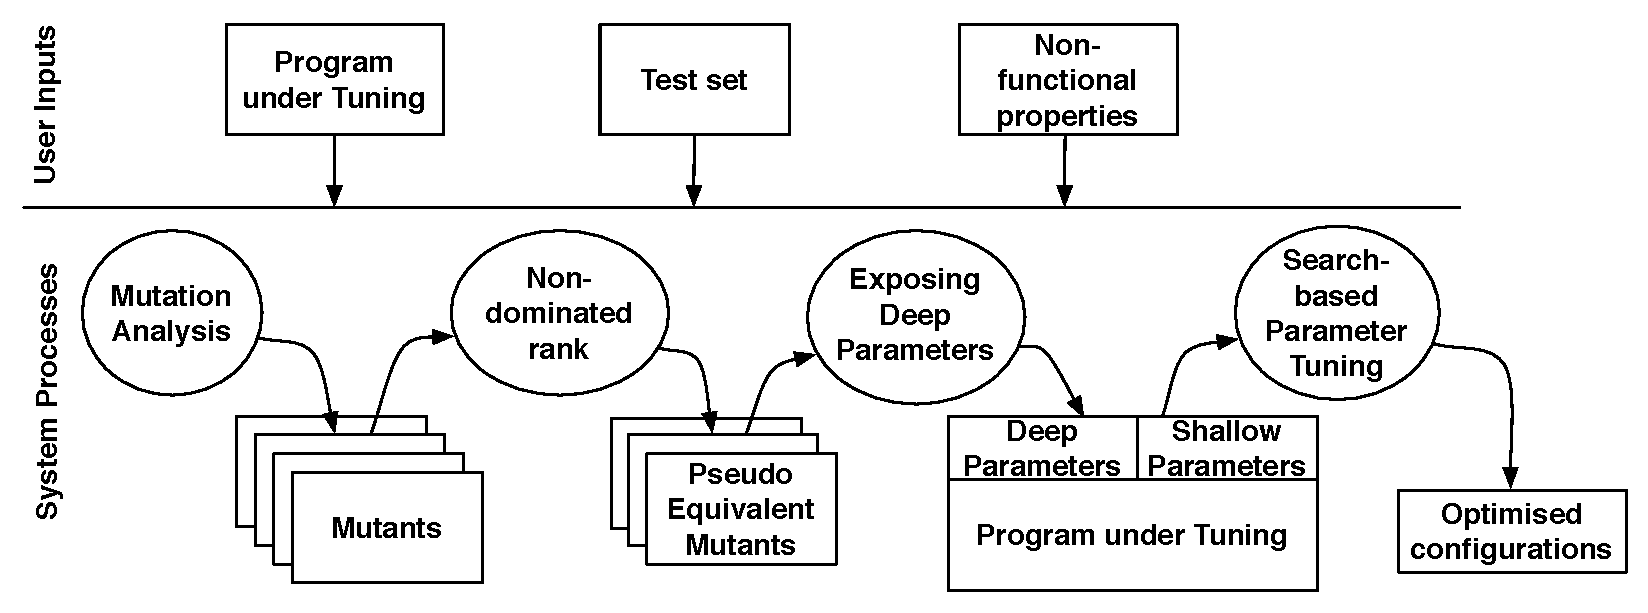
\includegraphics[width=6.2in]{pics/new_system}
\caption{Deep parameter optimisation workflow. It takes source code of a program, test suite and non-functional properties of interest as input, applies mutation analysis to identify most sensitive parts of the code, exposes deep parameters from them and optimise them}\label{system}
\end{figure*}

\subsection{Discovering locations for deep parameters}
\label{discovering}
The first step is to identify potential locations at which we could expose deep parameters. 
In our approach, we represent the input program as an abstract syntax tree and a potential location $L$ is an expression node of the AST. 
We want to find a set of locations $L_D$ such that when we tune the value of the expression at $L_D$, some non-functional properties of the program could be improved while the program retains the same functionality. 
%We use software testing to valid the functional behaviour of the program. 
%To valid the functional behaviour of the tuned program, we test the tuned program with the input test set and compare the output with the test output of the original program.
We use regression testing, with a suite of regression test data to check for regression of functionality correctness from the optimisation as with other Genetic Improvement approaches \cite{justyna2013, Langdon:2014:IMI:2576768.2598244}.

We use mutation analysis to automate the process of searching for locations $L_D$. Mutation analysis deliberately makes simple syntactic changes to the input program, to create a set of various version programs called mutants, each contains a different syntactic change \cite{5487526}. A transformation rule that generates a mutant from the input program is known as a mutation operator. By carefully choosing mutation operators, we can use mutants to simulate the effect of making changes at all potential locations $L$. Table \ref{tab:cmop} lists the operators we used to generate mutants, covering locations of constants, relational, logical and arithmetic expressions. 
To assess the quality of a mutant, we test each mutant against the input test set and record the values of the non-functional properties. If the result of running a mutant is different from the result of running the origianl program for any test data in the input test set, then the mutant is said to be ``killed'', otherwise it is said to have ``survived''. 

\begin{table*} [ht]
\caption{Selected mutation operators}
\label{tab:cmop} 
\begin{center}
\begin{tabular}{ | c | l | l |}
  \hline
  Mutation Operators & Brief Description & Details \\ 
\hline
  CRCR & Required constant replacement & Replace a scalar reference with constants $0, 1, -1$ \\
  OAAN & Arithmetic operator mutation & Replace $+, -, *, /, \%$ with each other \\
  OAAA & Arithmetic assignment mutation & Replace $+=, -=, *=, /=, \%=$ with each other \\
  OCNG & Logical context negation & Replace $expr$ with $!expr$ in selective and iterative statements\\
  OIDO & Increment/decrement mutation  & Replace $++x, --x, x++, x--$ with each other \\
  OLLN & Logical operator mutation  & Replace $\&\&, ||$ with each other \\ 
  OLNG & Logical negation & Replace \emph{x op y} with \emph{x op !y}, \emph{!x op y}, \emph{!(x op y)}\\
  ORRN & Relational operator mutation & Replace $>, >=, <, <=, ==$ with each other \\
  OBBA & Bitwise assignment mutation & Replace $\&=, |=$ with each other \\
  OBBN & Bitwise operator mutation & Replace $\&, |$ with each other \\
\hline
\end{tabular} 
\end{center} 
\end{table*} 

After all mutants are executed, we first filter out the killed mutants which fail to retain the functional behaviour.  Thus we only select pseudo equivalent mutants which preserve the behavious of the original program. A mutant is called \textbf{pseudo equivalent} with respect to a given test suite $T$ iff. it passes the regression test of $T$.
In practice, there are a large number of pseudo equivalent mutants \cite{5477100} generated and we only want to select a subset from them which represents the locations that could have the greatest impact on the non-functional properties of interests, and we also want to have a diverse set of choices.  
We achieve this by ranking the mutants based on their non-functional properties using the non-dominated sorting approach of the NSGAII algorithm \cite{996017}. Each mutant is assigned a Pareto Level value and a Crowd Distance value, where Pareto Level $n$ means a mutant will be on the Pareto Front after all the mutants with Pareto Level less than $n$ are removed, while Crowd Distance indicates how close a mutant is to its neighbours on the same Pareto Level. Specially, a mutant with Pareto Level $1$ means it's on the Pareto Front among all the mutants and has the priority to be considered first. A mutant is better than another in terms of non-dominated sorting if its Pareto Level is smaller or their Pareto Level is the same but the former is less crowded (bigger Crowd Distance) than the latter. After sorting all the mutants in terms of their non-functional properties, we apply a greedy algorithm to pick the first $k$ locations that could best influence the non-functional properties of the original, where $k$ is the desired number of Deep Parameters one wants to expose.

\subsection{Exposing deep parameters}
\label{exposing}
The second step is to expose deep parameters which allow users to modify the value of the expression at selected locations. Based on the type of mutation, we first classify the selected mutants into two sets. $Set$ 1 contains mutants generated from CRCR, OAAN, OAAA and OIDO operators, which simulate locations with non-logical expressions. $Set$ 2 contains mutants generated from the OCNG, OLLN, OLNG and ORRN operators, which simulate locations with logical expressions. 
Given an location $L$, $E_L$ is the expression at the location $L$, we use the following transformation rules to rewrite $E_L$ with a new parameter $v$.

\begin{equation}
 E_L \rightarrow \left\{
  \begin{array}{l l}
    (E_L + v) & \quad \text{if $L$ $\in$ Set 1}\\
    (E_L) \ xor \ v & \quad \text{if $L$ $\in$ Set 2}
    \end{array} \right.
\end{equation}

We use addition to affect the value of non-logical expression and exclusive or to affect the logical ones.
Finally we expose $v$ as a `public' parameter so that users can assign value to $v$ through parameter passing or APIs.

\subsection{Search-based parameter tuning}
\label{sec_nsgaii}

Although the exposed deep parameters can provide additional `knobs' \cite{Hoffmann:2011:DKR:1961296.1950390} to tune the program, they cannot completely substitute the shallow parameters of the program.  Thus, in this work, we propose to use both shallow parameters and deep parameters and tune them together using SBSE \cite{Harman:2007:CSF:1253532.1254729}. Because we are interested in multiple non-functional properties, a multi-objective Genetic Algorithm, NSGA II \cite{996017}, is applied to search for optimal values for both shallow and deep parameters.


We use an integer vector to represent the list of parameters under tuning. Each gene stores a solution value for one parameter. At each generation, our NSGAII first applies tournament selection followed by a uniform crossover and a uniform mutation operation. In this work our fitness functions are designed to capture two non-functional properties: execution time and memory consumption. To measure execution time, \emph{Glibc}'s \emph{wait4} system call is used to calculate the total CPU time consumed by the program. For memory consumption, we instrumented the program under tuning to record the high-water mark of the virtual memory consumption. This is due to the fact that the physical memory reported by OS is not always deterministic but depends on the workload and the OS. After fitness evaluation, a standard NSGA II non-dominated selection is applied to create the next generation. Finally, all non-dominating solutions in the final population are returned.


\section{Experiments}

In order to assess the improvement of our Deep Parameter Tuning approach, we compared our approach with the shallow parameter tuning approach and posed the following research questions: 
 

\begin{description}
 \item[RQ1] {\bf How much improvement can be obtained using the Shallow Parameter Turning approach? }
\end{description}

We asked RQ1 to provide us a baseline results against which to compare the results from our approach. To mimic a traditional Shallow Parameter Turning approach, we used the same NSGAII algorithm introduced in Section \ref{alg} to search for the default explicit parameters for Dlmalloc. To answer this question, we compared the performance of the optimised configuration found by the Shallow Parameter Turning approach with the default Dlmalloc configuration and a set of random generated configurations.  %The default Dlmalloc configuration is chosen by the developer of Dlmalloc and is believed can achieve a good performance on a wide range of programs. We 

\begin{description}
\item[RQ2] {\bf How much more improvement can be obtained using the Deep Parameter Turning approach? }
\end{description}

We ask the RQ2 to see how useful our approach is at find optimised configurations for the given non-functional properties. Our Deep Parameter Turning approach apply NSGAII to optimise both explicit and implicit parameters for Dlmalloc. Of course, should it turn out that the Shallow Parameter Turning approach can find better configuration than our approach, then our approach would not be needed. 

\begin{description}
\item[RQ3] {\bf Do we see evidence that our Deep Parameter Tuning approach can expose implicit parameters which are meaningful to human developer? }
\end{description} 

Should it turn out that the Deep Parameter Tuning approach performs well, achieving much improvement than the Shallow Parameter Tuning approach, then we have evidence to suggest that the mutation based sensitivity analyse used in our approach is able to locate the inner expressions or variables which are sensitive to the given non-functional properties. However, do these inner expressions or variables also make sense to software developer? To answer this research question, we manually investigate the exposed variable and try learn why tuning these parameter can make Dlmalloc more efficient.  

\subsection{Experiment Setup}


\begin{table}[htbp]
\centering
\caption{subject applications}
\label{tab_sub_app}
\resizebox{0.5\textwidth}{!}{
\begin{tabular}{|c|c|c|l|}
\hline
Name & Loc & No. of tests & Type \\
\hline
espresso & 13256 & 19 & Digital electronic gate circuits simplification\\
\hline
cfrac & 6040 & 2 & Big integer factorization\\
\hline
space & 5846 & 3 & Astronautics interpretation\\
\hline
gawk & 45241 & 20 & String processing\\
\hline
\end{tabular}}
\end{table}

For our evaluation, we selected four real world applications: \emph{espresso}, \emph{space}, \emph{cfrac} and \emph{gawk}. \emph{Espresso} is a fast application for simplying complex digital electronic gate circuits and \emph{cfrac} is a factorization application for big integers. We obtain these two applications from the benchmarks of the \emph{DieHard} project\cite{}. \emph{Space} is a well known real world application in astronautics. We obtain this program from the SIR repository \cite{}. \emph{Gawk} is the GNU \emph{awk} implementation for strings processing. We collect this application from the GNU archives \cite{}

Although turning parameter of malloc is less likely to change the behaviour of our subjects under optimise directly, some combination of unusual parameters' values could also crush a subject system. To make sure the configuration generated by our approach always prodcue the same results as the default configuration, we use the number of passed tests as an addtional hard constraints. We used the tests from the \emph{DieHard} project for \emph{Espresso} and \emph{cfrac} and the tests from SIR for \emph{Space}. These tests are designed by programmer and achieve high branche coverage. We mannully generated tests for \emph{awk}, which achieves ** branch coverage. 

All experiments were carried out on a desktop computer with a quad core 3.4GHz CPU and 7.7 GB memory runing 64-bit Ubuntu 13.10. We used \emph{dlmalloc} version 2.8.6 as our base allocator. It was compiled with gcc 4.8.1 with -O3 option. In order to capture the execution time and memory consuming precisly, we adapt developed our own performance tool to measure the CPU time and maxium vitural memory consumption (see Section \label{}) The tool is publicly available at www.fan.put.a.link.later.



\section{Results}
\label{sec_results}

% FIXME: If you can, put a paragraph summarizing this section here so that
% the section heading is not immediately followed by the subsection heading.
% Fan wrote the following.

We formalise the metrics we use to compare multi-objective optimisation approaches in this section.
The results are presented in Section~\ref{sec_answers}, and are used to answer the \textbf{RQ}s.

\subsection{Metrics}
\label{sec_matrics}

To investigate RQ1 and RQ2, we collect the non-dominated set of solutions from each algorithm for 20 runs, and report it in an attainment surface as introduced by Fonseca~\cite{attainment_surface:1996}. To quantitatively compare the quality of each algorithm, we calculate Hypervolume and Contribution indicators to assess the multi-objective Pareto Front.

\textbf{Hypervolume}: The Hypervolume indicator~\cite{797969} measures the space dominated by the solutions. It is defined as the hypervolume of the union of hypercubes dominated by each solution on the Front. The bigger the Hypervolume is, the larger the area dominated by the Pareto Front in the objective space is, and thus the better the performance is.

\textbf{Contribution}: Since there is no way to know the true Pareto Front, we use the non-dominated set of joint solutions from all experiments to approximate the true Pareto Front, forming a `reference' front. The Contribution indicator represents the ratio of solutions on the reference front that are found by a given algorithm. A higher ratio indicates a more successful search. 

To allow comparison across subject programs, objectives are normalised to the original performance of each subject.


\subsection{Answers to RQs}
\label{sec_answers}

\newcommand{\shallow}{Sha}
\newcommand{\all}{All}
\newcommand{\randomsearch}{Rand}
\newcommand{\nsgaii}{NSGA}
\newcommand{\sr}{\emph{\shallow\randomsearch}}
\newcommand{\sn}{\emph{\shallow\nsgaii}}
\newcommand{\dr}{\emph{\all\randomsearch}}
\newcommand{\dn}{\emph{\all\nsgaii}}

For brevity we use \emph{\shallow} to refer to shallow parameters and \emph{\all} to refer to all parameters including shallow and deep parameters, followed by \emph{\randomsearch} or \emph{\nsgaii} to indicate the search method used (random search or NSGA-II). For example, \sn{} refers to using NSGA-II to search for better values for shallow parameters.
%In subsequent graphs, the performance of the original program always locates at (1, 1) since all the performance is normalised to it.

\begin{figure*}[htb]
	\centering
	\subfigure[espresso]{
		\label{fig_attainment_espresso}
		\scalebox{1}{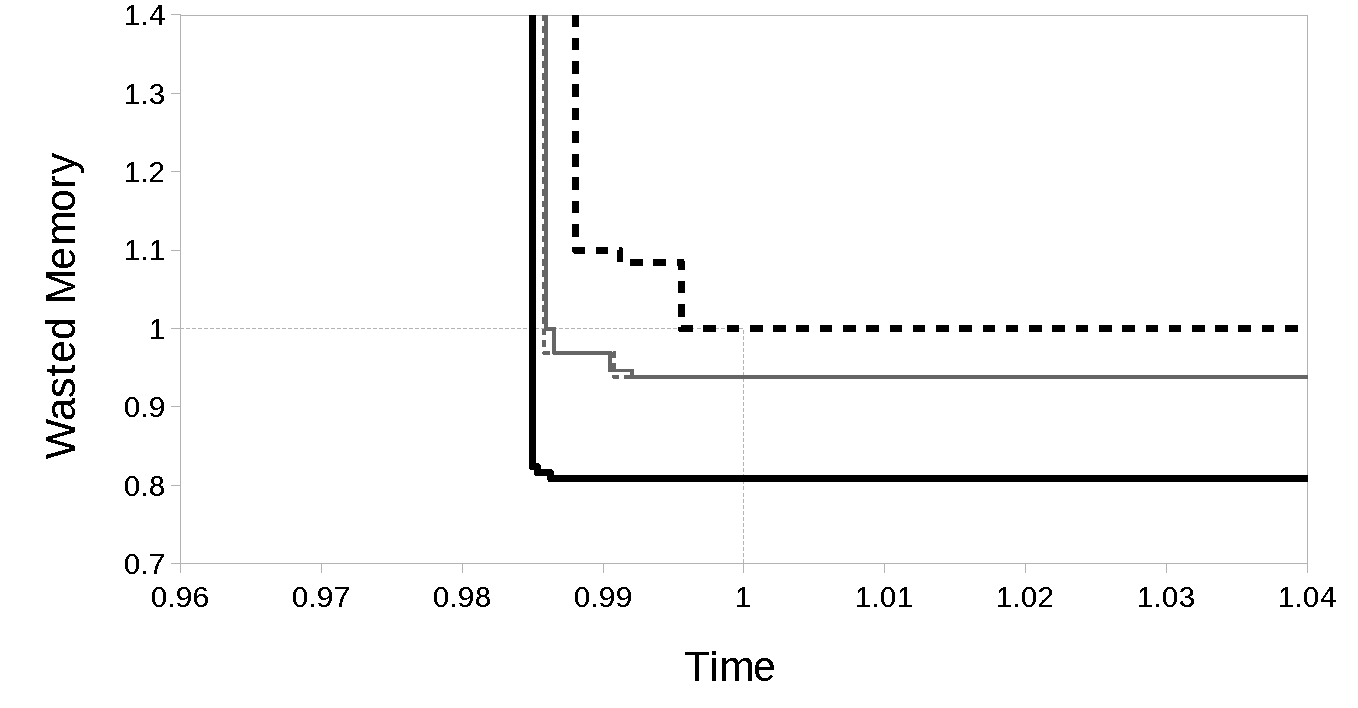
\includegraphics[width=0.47\textwidth]{espresso_attainment_pdf}}
	}
	\subfigure[gawk]{
		\label{fig_attainment_gawk}
		\scalebox{1}{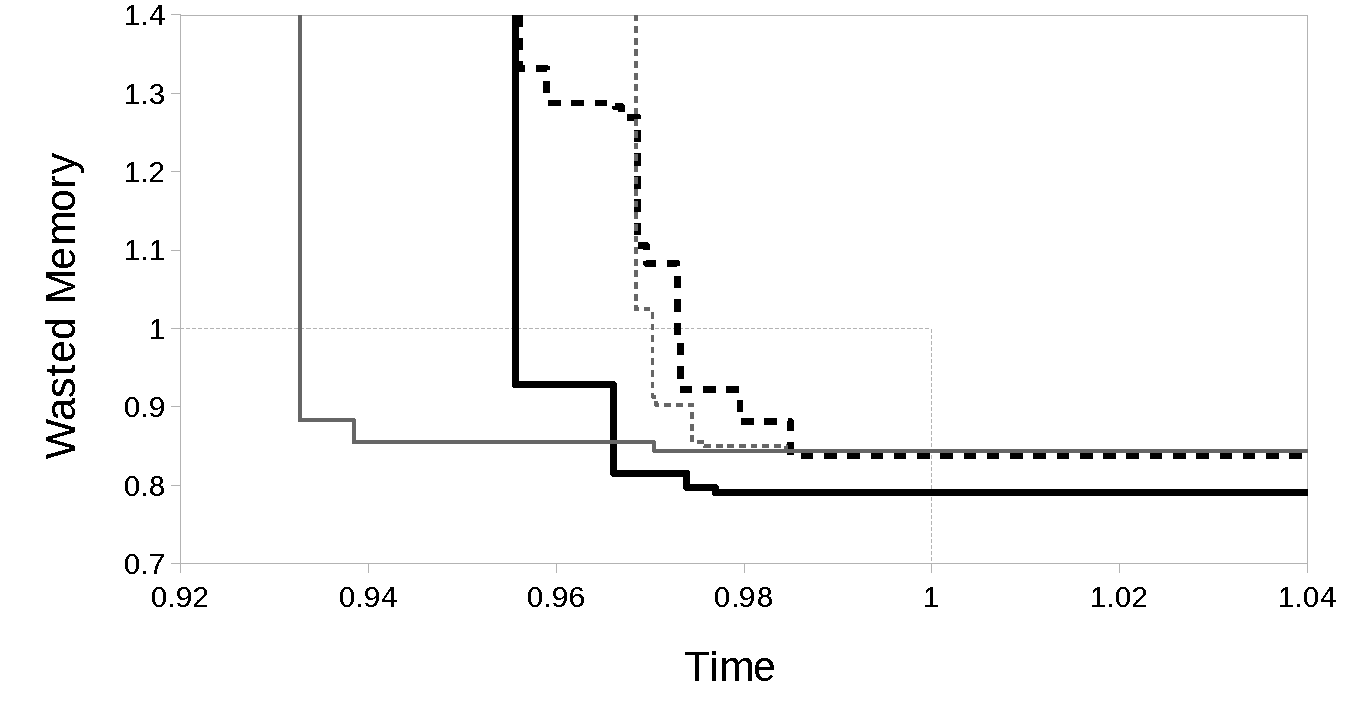
\includegraphics[width=0.47\textwidth]{gawk_attainment_pdf}}
	}
	\subfigure[flex]{
		\label{fig_attainment_flex}
		\scalebox{1}{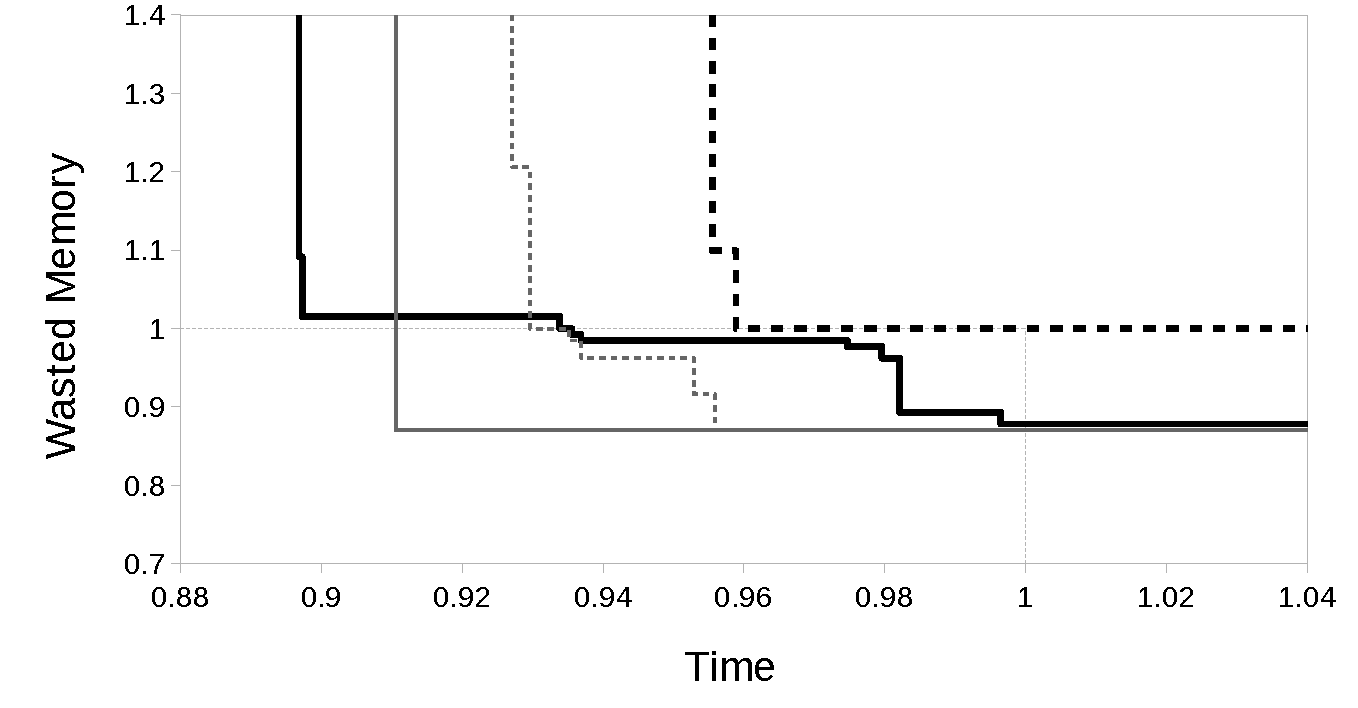
\includegraphics[width=0.47\textwidth]{flex_attainment_pdf}}
	}
	\subfigure[sed]{
		\label{fig_attainment_sed}
		\scalebox{1}{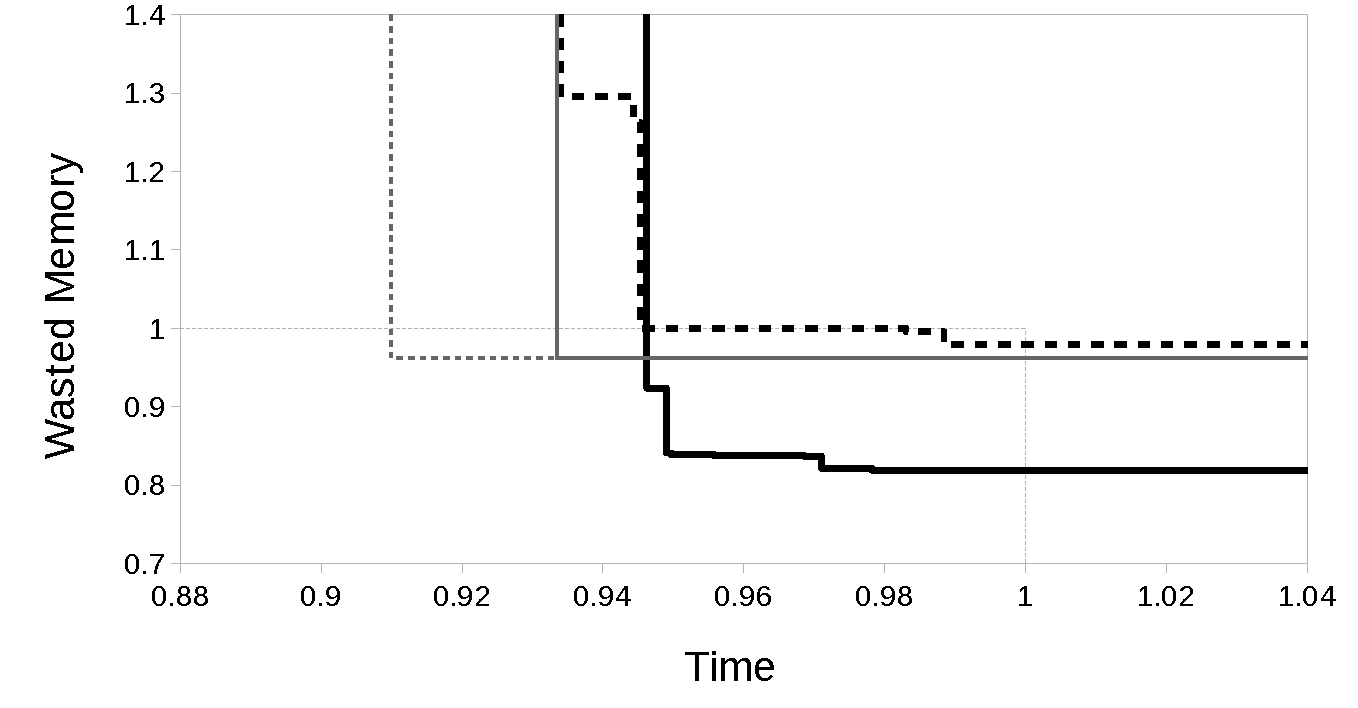
\includegraphics[width=0.47\textwidth]{sed_attainment_pdf}}
	}
	\subfigure{
		\label{fig_attainment_legend}
		
\includegraphics[width=0.45\textwidth]{attainment_legend_pdf}
	}
	\vspace{-1.5em}
	\caption{Combined best solutions from the results of \sr{}, \sn{}, \dr{}, \dn{} over 20 runs for each application. Lower and lefthand solutions dominate high and righthand solutions. `Wasted' memory is memory that is used but not needed.}\label{fig_attainment}

\end{figure*}

To answer RQ1 and RQ2, we first report the 0\%-attainment surfaces (the `reference front' that combines best solutions over all runs) of the results of \sr{}, \sn{}, \dr{} and \dn{} on all subjects in Figure~\ref{fig_attainment}. The solutions are plotted according to their execution time and memory usage (at the `high-water-mark') compared to the original performance. Specially, the original always lies at (1, 1) and is pinpointed by light grey dashed lines. The high-water-mark is our primary target since the remaining non-wasted memory is needed and thus cannot be reduced. 
The figure shows that all algorithms can reduce time or memory consumption without reducing the other objective, implying that the default configuration of \emph{dlmalloc} is not optimal for any application considered. This finding motivates the use of SBSE for tuning memory allocators. In three subjects (\emph{espresso}, \emph{gawk} and \emph{sed}), \dn{} outperforms the other three on memory objective. In terms of time, no algorithm is strictly better and each has its own strengths on different subjects. 
%In Figure~\ref{fig_shallow_random}, we can see that Shallow algorithm is better than Random on subject \emph{sed}, while they are incomparable on the other three subjects. In Figure~\ref{fig_deep_shallow}, Deep algorithm is better than Shallow on three out of four subjects: \emph{espresso}, \emph{gawk}, \emph{sed}, while incomparable on subject \emph{flex}. Notice that unlike other three subjects, Deep can not find solutions have better performance on memory consumption on subject \emph{flex}, and both Shallow and Deep algorithm perform as good as Random, it implies that the optimal solution is very easy to find in the search space. So any search algorithm would fail to ourperform Random search on this special case.

We calculated the Hypervolume and Contribution indicator of each algorithm on every subject, and report them in Figure~\ref{fig_hypervolume} and~\ref{fig_contribution} respectively for all 20 runs. 
In Figure~\ref{fig_hypervolume}, all the values are normalised to the hypervolume of the 0\% attainment reference front, and the closer the value to $1$ is, the better the result is. It is clear that \dn{} outperforms the others on subject \emph{espresso} and \emph{sed} while it performs poorly on subject \emph{flex}, and on subject \emph{gawk} the best value reached by \dn{} is better than that of the others.
%In terms of Hypervolume indicator, Deep algorithm performs the best in general, with an exception on subject \emph{flex}. Shallow algorithm is statistically better than Random on subject \emph{sed}, but there is no significant difference between them on the other three subjects. 
In terms of Contribution, the performance of all algorithms is similar to that of Hypervolume. In general \dn{} is no worse than other algorithms on all subjects but \emph{flex}, where \sn{} has the highest Contribution value.
 
\begin{figure}[htbp]
	\centering
	\subfigure[espresso]{
		\label{fig_hypervolume_espresso}
		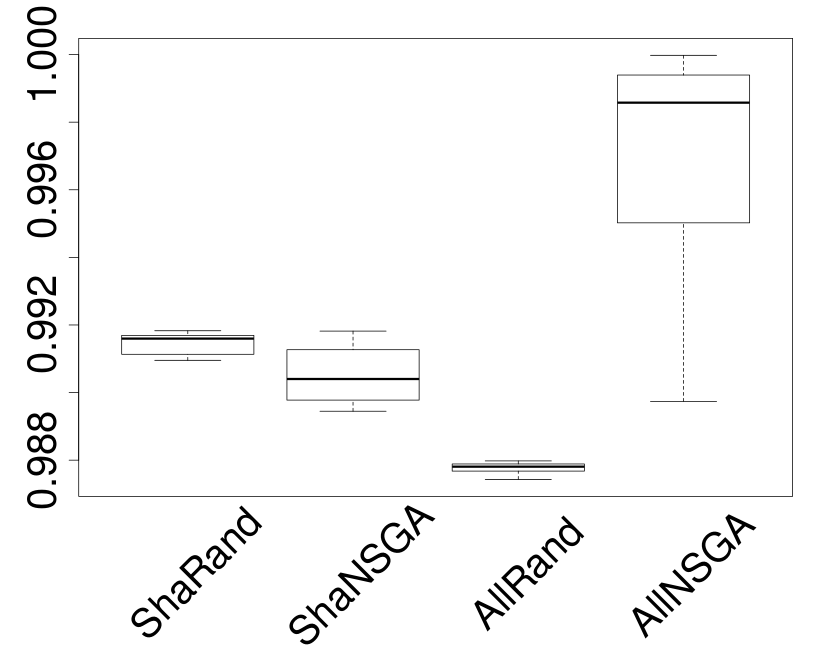
\includegraphics[width=0.22\textwidth]{espresso_hypervolume}
	}
	\subfigure[gawk]{
		\label{fig_hypervolume_gawk}
		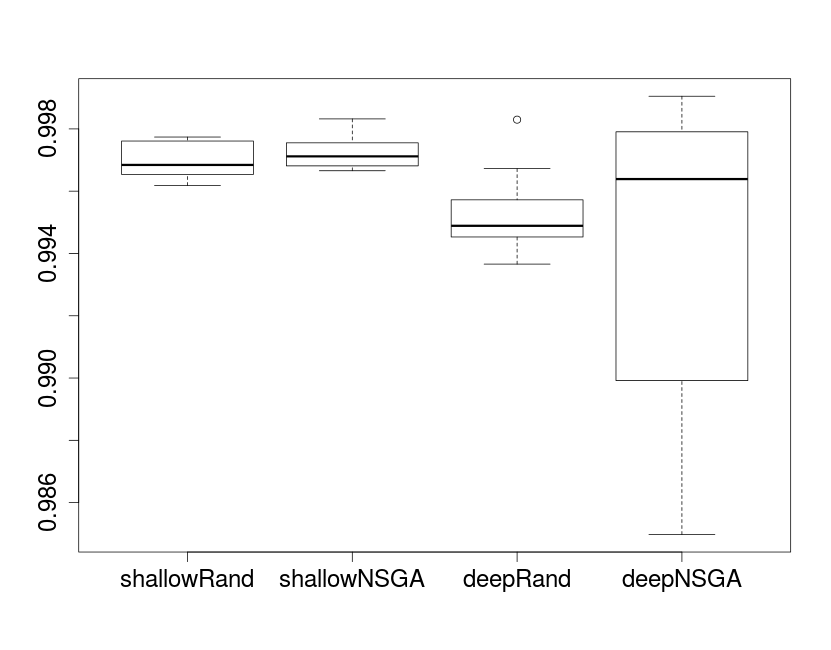
\includegraphics[width=0.22\textwidth]{gawk_hypervolume}
	}
	\subfigure[flex]{
		\label{fig_hypervolume_flex}
		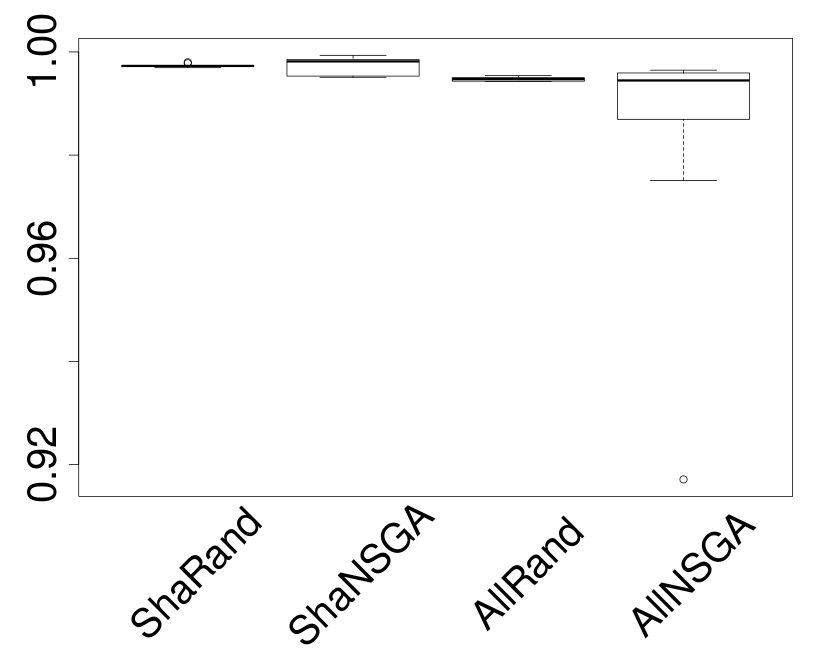
\includegraphics[width=0.22\textwidth]{flex_hypervolume}
	}
	\subfigure[sed]{
		\label{fig_hypervolume_sed}
		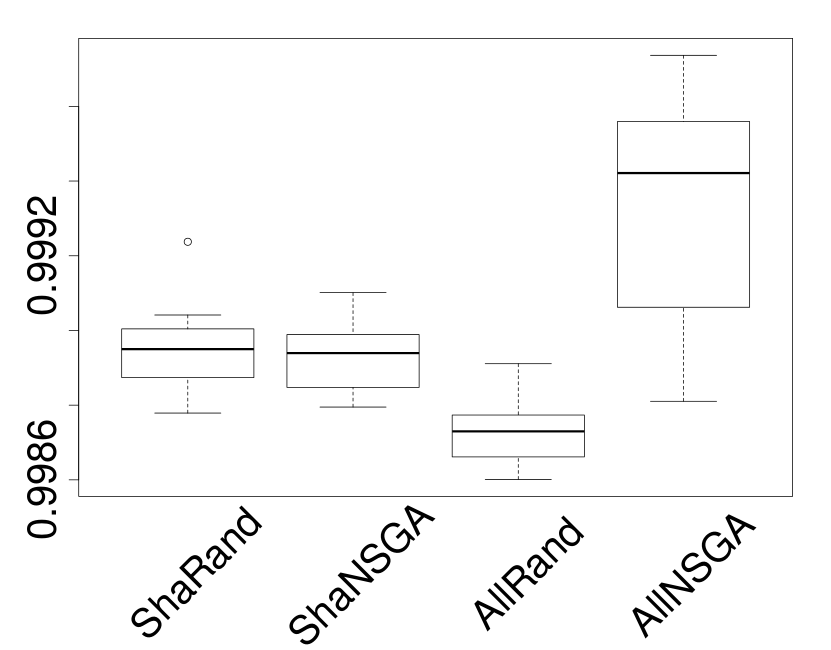
\includegraphics[width=0.22\textwidth]{sed_hypervolume}
	}
	\vspace{-1.2em}
	\caption{Hypervolume indicator of \sr{}, \sn{}, \dr{}, \dn{} on all subjects. Larger values are better.}\label{fig_hypervolume}
	\vspace{-1em}
\end{figure}

\begin{figure}[htbp]
	\centering
	\subfigure[espresso]{
		\label{fig_contribution_espresso}
		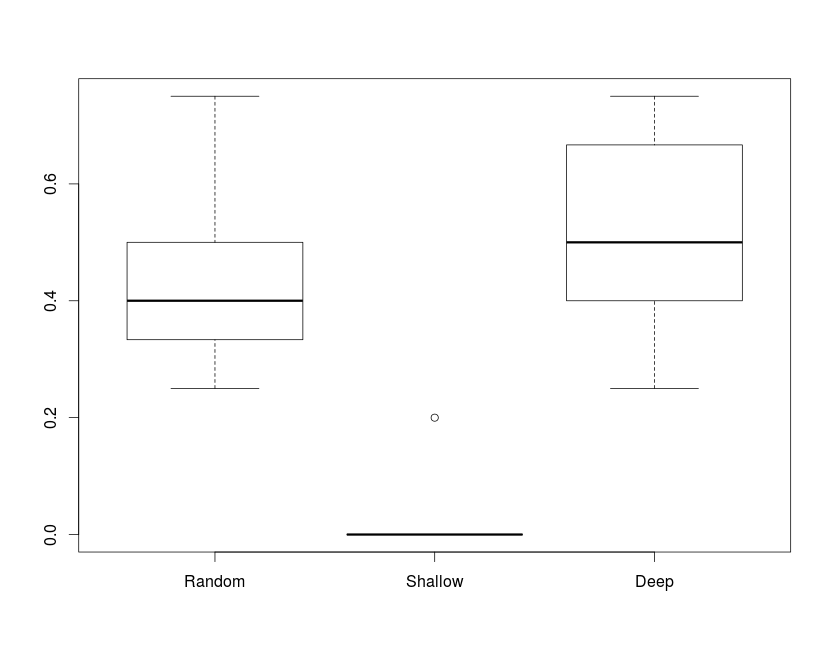
\includegraphics[width=0.22\textwidth]{espresso_contribution}
	}
	\subfigure[gawk]{
		\label{fig_contribution_gawk}
		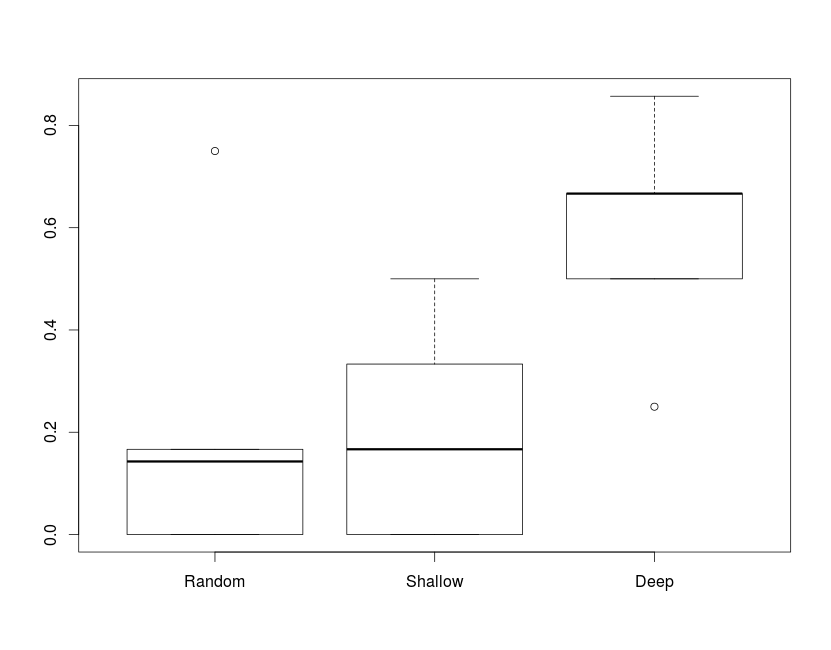
\includegraphics[width=0.22\textwidth]{gawk_contribution}
	}
	\subfigure[flex]{
		\label{fig_contribution_flex}
		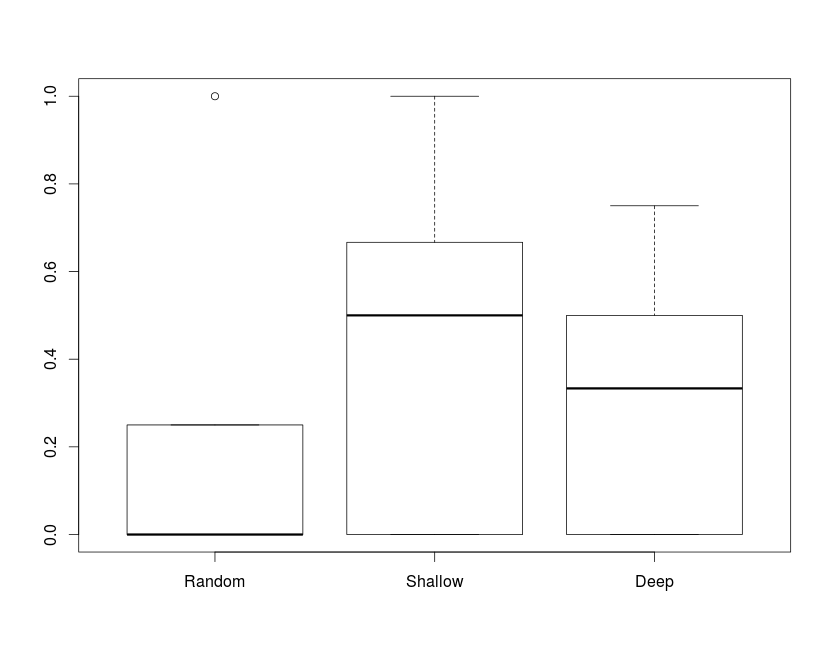
\includegraphics[width=0.22\textwidth]{flex_contribution}
	}
	\subfigure[sed]{
		\label{fig_contribution_sed}
		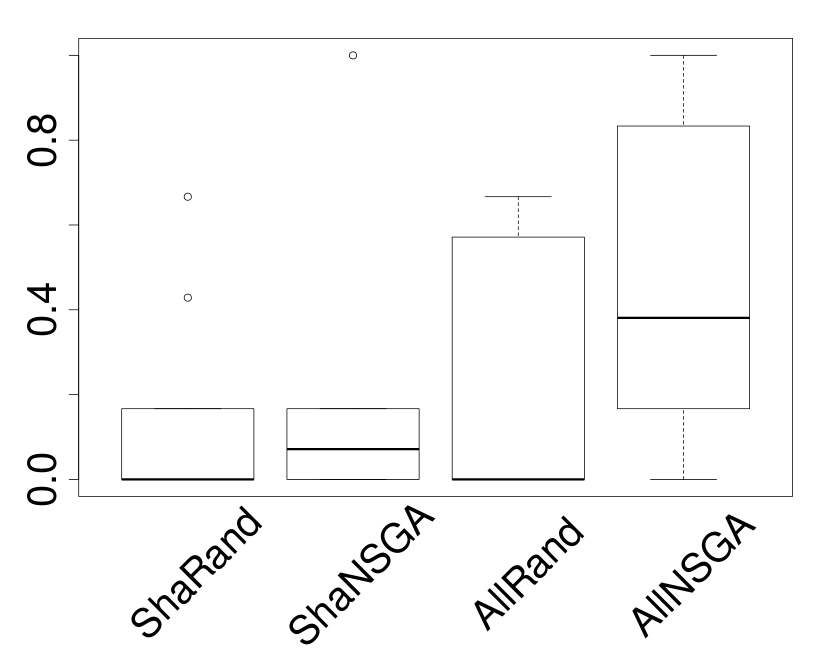
\includegraphics[width=0.22\textwidth]{sed_contribution}
	}
	\vspace{-1.2em}
	\caption{Contribution indicator of \sr{}, \sn{}, \dr{}, \dn{} on all subjects. Larger values are better.}\label{fig_contribution}
	\vspace{-1em}
\end{figure}

\begin{figure}[htb]
	\centering
	\subfigure[espresso]{
		\label{fig_best_time_espresso}
		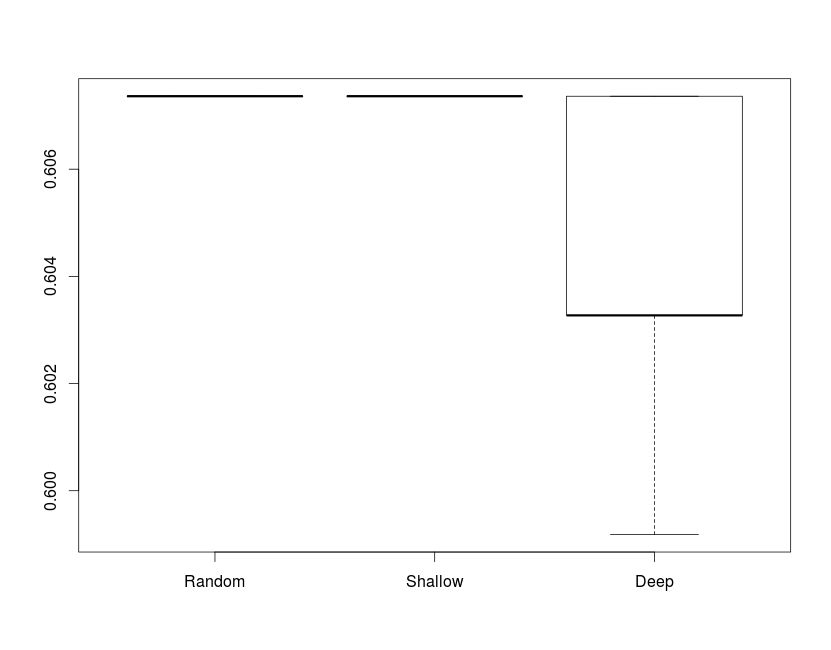
\includegraphics[width=0.22\textwidth]{espresso_best_memory}
	}
	\subfigure[gawk]{
		\label{fig_best_time_gawk}
		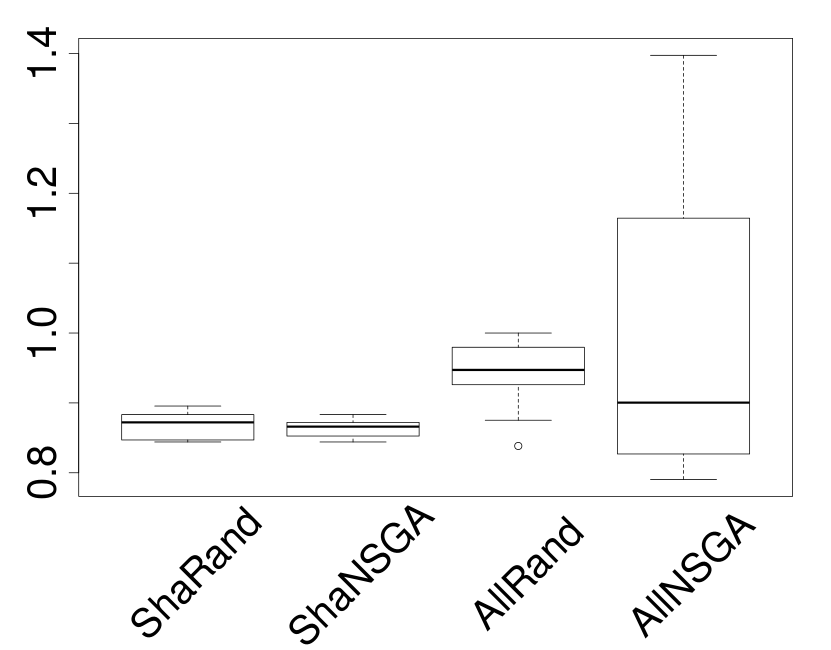
\includegraphics[width=0.22\textwidth]{gawk_best_memory}
	}
	\subfigure[flex]{
		\label{fig_best_time_flex}
		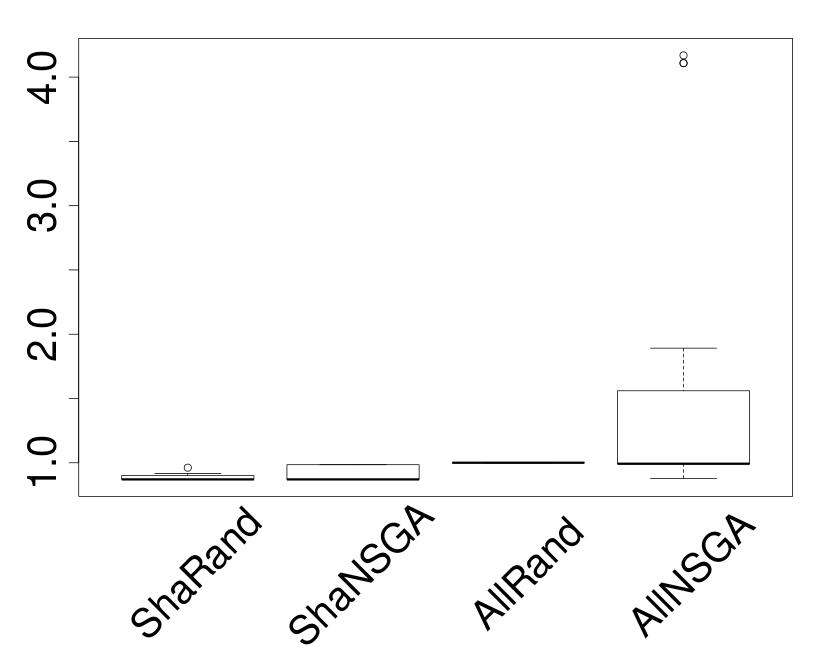
\includegraphics[width=0.22\textwidth]{flex_best_memory}
	}
	\subfigure[sed]{
		\label{fig_best_time_sed}
		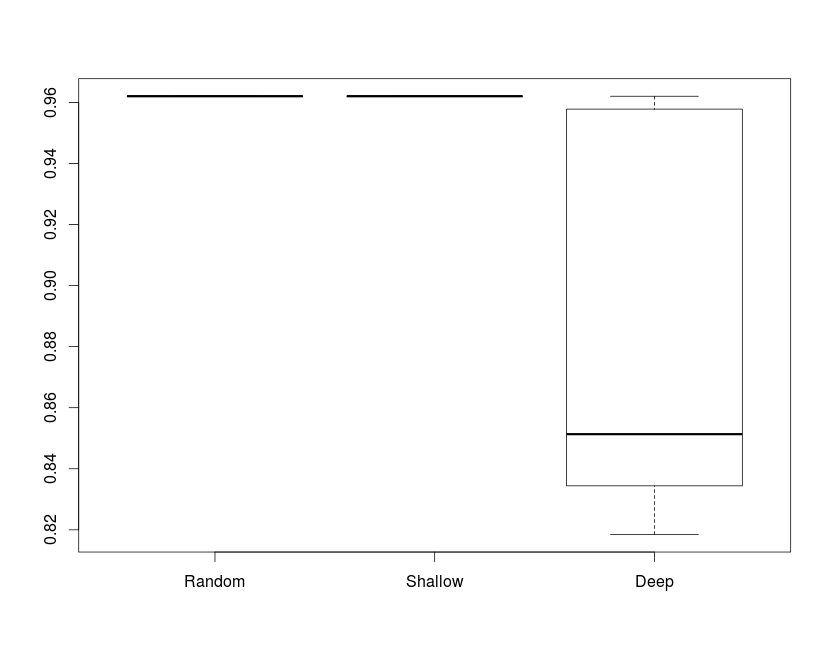
\includegraphics[width=0.22\textwidth]{sed_best_memory}
	}
	\vspace{-1.2em}
	\caption{The least memory consumption found by each algorithm. Smaller numbers are better.}\label{fig_best_memory}
	\vspace{-1em}
\end{figure}

Since \dn{} is good at finding better performance on memory consumption, we report the most memory-saving performance found by each algorithm of each of 20 runs in Figure~\ref{fig_best_memory}. On subject \emph{espresso} and \emph{sed}, \dn{} finds more memory reduction than the other approaches. On \emph{gawk}, it does not perform as consistently, but can also find more memory reduction than other approaches in the best case. 
% FIXME: What does ``potential to do so'' mean here? Please clarify this
% analysis.
% Fan was trying to say, for gawk, though on average AllNSGA doesn't perform as good and stable as other approaches,
% but can occationally outperform other approaches.

%Statistics tests are applied to Hypervolume, Contribution and Best-Memory-Reduction over all subjects.
%We choose Wilcoxon \emph{U}-test because we don't make any assumption on the distributions and the experiments are not paired.
%Considering four approaches on four subjects, we apply Bonferroni Correction (16 tests) to draw conservative conclusions.
%For those \emph{p}-values less than $5\%/16=0.3125\%$, we apply
%Vargha-Delaney effect size measure ($\hat{A}_{12}$) and report the effect sizes in Table~\ref{table_p_value}.
%The effect sizes are all large (effect size larger than $0.79$ or less than $0.21$).

Inferential statistical tests were applied to the Hypervolume, Contribution and Best-Memory-Reduction results over all subjects.
We used the Mann-Whitney-Wilcoxon \emph{U}-test since we make no assumptions about results distributions and apply a Bonferroni Correction (catering for 16 total statistical tests) to draw conservative conclusions with no risk of Type 1 error.
For those \emph{p}-values less than $0.05/16=0.003125$, we apply the
Vargha-Delaney ($\hat{A}_{12}$) effect size measure (see Table~\ref{table_p_value}).
The effect sizes are all large (either above $0.79$ or below $0.21$).

In all experiments involving \emph{\all{}*} we generated and evaluated invalid
configurations (i.e., those that that cause the program to crash). However,
this issue is not specific to our deep-parameter approach: 
surprisingly, even by just tuning the programmer-specified shallow parameters 
(\sr{} and \sn{} optimisations) we {\em also} encounter (and discard) some
configurations that crash the program.
%Unlike shallow parameters, deep parameters are exposed from internal
%sub-expressions that were not monitored or protected by the programmers,
%hence they are expected to cause crashes more often. As a result, the valid
%configurations are sparser in the search space. 
This suggests that SBSE memory allocator tuning can be used as a search based testing technique \cite{mh:icst14-keynote}.
Without any guidance, \dr{}
finds valid configurations less often than \sr{}, and thus requires more
optimisation time than \sr{}. Holding the searches to the same budget means
that \dn{}, which must explore a higher search space, will exhibit a higher
variance. 
% This is also the reason why the performance of \dn{} is not alway
% stable on all subjects. 
Despite this more challenging search space, exposing and optimising deep
parameters still allows \dn{} to find better configurations
than \sn{}.

\begin{table*}[htb]
\centering
\caption{Vargha-Delaney effect sizes of Hypervolume, Contribution and Best Memory Reduction for any two of the approaches on all subjects. Only the effect sizes of tests with \emph{p}-value less than $5\%/16=0.3125\%$ are reported.}
\label{table_p_value}
\resizebox{0.85\textwidth}{!}{
\begin{tabular}{|l|l|r|r|r|r|r|r|r|r|r|r|r|r|}
\hline
\multicolumn{2}{|l|}{\multirow{2}{*}{Comparing Approachs}} & \multicolumn{4}{c|}{Hypervolume}                                                                             & \multicolumn{4}{c|}{Contribution}                                                                            & \multicolumn{4}{c|}{Best Memory Reduction}                                                                   \\ \cline{3-14} 
\multicolumn{2}{|l|}{}                           & \multicolumn{1}{c|}{\emph{espresso}} & \multicolumn{1}{c|}{\emph{gawk}} & \multicolumn{1}{c|}{\emph{flex}} & \multicolumn{1}{c|}{\emph{sed}} & \multicolumn{1}{c|}{\emph{espresso}} & \multicolumn{1}{c|}{\emph{gawk}} & \multicolumn{1}{c|}{\emph{flex}} & \multicolumn{1}{c|}{\emph{sed}} & \multicolumn{1}{c|}{\emph{espresso}} & \multicolumn{1}{c|}{\emph{gawk}} & \multicolumn{1}{c|}{\emph{flex}} & \multicolumn{1}{c|}{\emph{sed}} \\ \hline
\multirow{3}{*}{\dn{}}              & \dr{}        & 1.000                     & --                        & --                        & 0.975                    & 0.859                     & --                        & --                        & 0.835                    & 0.000                     & --                        & --                        & 0.000                    \\
                                   & \sn{}        & 0.935                     & --                        & 0.105                     & 0.808                    & 0.868                     & --                        & 0.191                     & 0.868                    & 0.063                     & --                        & 0.950                     & 0.050                    \\
                                   & \sr{}        & 0.900                     & --                        & 0.035                     & 0.785                    & 0.814                     & --                        & --                        & 0.875                    & 0.100                     & --                        & 0.979                     & 0.050                    \\ \hline
\multirow{2}{*}{\dr{}}              & \sn{}        & 0.000                     & 0.053                     & 0.038                     & 0.045                    & --                        & --                        & 0.144                     & --                       & 1.000                     & 0.940                     & 1.000                     & 1.000                    \\
                                   & \sr{}        & 0.000                     & 0.070                     & 0.000                     & 0.040                    & --                        & --                        & --                        & --                       & 1.000                     & 0.928                     & 1.000                     & 1.000                    \\ \hline
\multicolumn{1}{|c|}{\sn{}}         & \sr{}        & 0.198                     & --                        & --                        & --                       & --                        & --                        & --                        & --                       & 0.800                     & --                        & --                        & --                       \\ \hline
\end{tabular}
}
\vspace{-1.5em}
\end{table*}

To enable a more quantitative look at maximal time and memory savings, we
examine the extreme performance observed in our experiments. We report
those that have the best performance on
one objective, even at the cost of reducing performance on the other
objective, found by each
algorithm on each subject and summarise them in Table~\ref{table_best_time_memory}.
Some of these results are significant
departures from the original and are thus not plotted in Figure~\ref{fig_attainment}. 

\begin{table*}[htb]
\centering
\caption{Best reduction of time or memory (separately) found by each algorithm}
\label{table_best_time_memory}
\resizebox{\textwidth}{!}{
\begin{tabular}{|c|r|r|r|r|r|r|r|r|r|r|}
\hline
\multirow{2}{*}{Subject} & \multicolumn{1}{c|}{\multirow{2}{*}{\begin{tabular}[c]{@{}c@{}}Time\\ Original (s)\end{tabular}}} & \multicolumn{4}{c|}{Time Reduction (\%)} & \multicolumn{1}{c|}{\multirow{2}{*}{\begin{tabular}[c]{@{}c@{}}Memory Original\\ (Peak/Wasted KB)\end{tabular}}} & \multicolumn{4}{c|}{Wasted Memory Reduction (\%)} \\ \cline{3-6} \cline{8-11} 
                         & \multicolumn{1}{c|}{}                                                                               & \sr{}  & \sn{}  & \dr{}  & \dn{} & \multicolumn{1}{c|}{}                                                                                            & \sr{}    & \sn{}    & \dr{}    & \dn{}    \\ \hline
\emph{espresso}                 & 7.24                                                                                                & 1.4      & 1.4      & 1.5     & 1.5     & 3500/521                                                                                                         & 6.1        & 6.1        & 0          & 19.2       \\ %\hline
\emph{gawk}                     & 3.43                                                                                                & 3.2      & 6.7      & 4.4      & 4.4     & 29680/3552                                                                                                       & 15.6       & 15.6       & 16.2       & 20.9       \\ %\hline
\emph{flex}                     & 0.13                                                                                                & 7.9      & 10.0      & 6.2      & 11.6    & 10816/525                                                                                                        & 13.0       & 13.0       & 0          & 12.2        \\ %\hline
\emph{sed}                      & 0.25                                                                                                & 9.4      & 7.0      & 7.0      & 5.4     & 7048/948                                                                                                         & 3.8        & 3.8        & 2.1          & 17.9       \\ \hline
\end{tabular}
}
\vspace{-3mm}
\end{table*}

To answer RQ3, we provide the average optimisation computation time for each of the apporaches in Table~\ref{table_computation_time}. Recall that \dr{} generates and evaluates numerous invalid configurations. However, since crashing or incorrect mutants can be discarded immediately, the computation time of \dr{} is the lowest among all approaches (given a fixed budget in terms of mutants considered). Similarly, \dn{} generates invalid configurations more often than \sn{}, so it costs less computation time than \sn{}. Taking the deep parameter discovery time into account, \dn{} requires slightly more time than \sn{} does, and the percentage of the extra computation time is reported in the last column of Table~\ref{table_computation_time}. Ultimately, \dn{} requires at most 18\% more computation time than \sn{} (on \emph{espresso}), but requires only 0.7\% more computation time on \emph{flex}, on which \dn{} does not perform as well as \sn{}. Overall, since this optimisation step is a compile-time rather than run-time cost and can be done before deployment, we view the benefits of deep parameter optimisation as significantly outweighing their slight additional optimisation time cost.

\begin{table}[h]
\centering
\vspace{-1.4em}
\caption{Computation Cost in Time}
\label{table_computation_time}
\resizebox{0.47\textwidth}{!}{
\begin{tabular}{|c|r|r|r|r|r|r|}
\hline
\multirow{2}{*}{Subject} & \multicolumn{4}{c|}{Optimisation Time (h)}                                                                        & \multicolumn{1}{c|}{\multirow{2}{*}{\begin{tabular}[c]{@{}c@{}}Exposing\\ Time (h)\end{tabular}}} & \multicolumn{1}{c|}{\multirow{2}{*}{\begin{tabular}[p{2cm}]{@{}c@{}}Extra Time Needed\\ for \emph{*\nsgaii} (\%)\end{tabular}}} \\ \cline{2-5}
                         & \multicolumn{1}{c|}{\sr{}} & \multicolumn{1}{c|}{\sn{}} & \multicolumn{1}{c|}{\dr{}} & \multicolumn{1}{c|}{\dn{}} & \multicolumn{1}{c|}{}                                                                             & \multicolumn{1}{c|}{}                                                                                                           \\ \hline
\emph{espresso}                 & 39.7      & 46.4     & 9.0      & 39.3     & 12.5                                                                                                    & 18.5                                                                                                                          \\ %\hline
\emph{gawk}                     & 22.7      & 18.4     & 13.9     & 16.4     & 5.4                                                                                                     & 11.7                                                                                                                          \\ %\hline
\emph{flex}                     & 7.7       & 6.3      & 5.3      & 5.0      & 1.3                                                                                                     & 0.7                                                                                                                           \\ %\hline
\emph{sed}                      & 9.4       & 7.6      & 5.9      & 6.6      & 1.9                                                                                                     & 12.6                                                                                                                          \\ \hline
\end{tabular}
}
\vspace{-1em}
\end{table}



\subsection{Threats to Validity}

\textbf{Internal Validity}  When exposing deep parameters, we used a mutation-based sensitivity analysis because of its advantages in terms of efficiency and automation. Whether it is the best way to expose deep parameters remains to be proven. In addition, we have not formally investigated the relative merits of the Mutation Operators used. Intuitively, our Mutation Operators change a constant or an operator in an expression, and thus are likely to change the values of expressions to different degrees, allowing us to capture the sensitivity of that program's non-functional behaviour to the value of that expression. Any lack of efficacy of these Mutation Operators at capturing sensitivity information introduces a threat to the effectiveness of our approach. A formal evaluation of mutation operators for deep parameter tuning remains as future work.

Another threat to the internal validity is that the execution time measured
may depend on the workload of the machine. We mitigate this threat by
 averaging the execution time of 10 trials on an otherwise-unloaded machine. 
% FIXME: I thought is was 20 trials?
% Fan says, when each configuration of dlmalloc is evaluated, the execution time is evaluated 10 times
% and the mean of 10 is used as one objective. But 20 runs means the whole optimisation process
% with 300 generations is repeated 20 times.

\textbf{External Validity}  Our choice of benchmark programs and their
associated test suites influences the generality of our results. 
Even a good test suite that achieves high branch coverage, for
example, could still differ from real world
inputs, in which case the optimised configuration over this test suite may
neither achieve the best performance nor retain required functionality.
We attempt to mitigate this threat by including two subjects (\emph{flex} and \emph{sed})
from the SIR repository~\cite{SIR2005}. These subjects come with
sets of high quality test suites, which achieve multiple adequacy 
testing criteria.
% FIXME (talk about SIR and how awesome the test suites are).
% Yue added the sentences at the end.

Another aspect of generality is whether these results hold on other
applications. We attempt to mitigate this threat by selecting subject
applications from different fields, but our results
may not generalize beyond these benchmarks. 
% Currently we can safely claim that our approach works on three
% applications under test in this paper, but because of the wide range of
% where these applications come from, the approach is likely to be
% generalized on other applications.

\section{Related Work}

Some embedded systems, especially those executing multimedia applications, suffer from massive memory usage and limited resources. Risco-Martin et al\cite{Risco-Martin:2009:ODM:1569901.1570116}\cite{RiscoMartin2010572} decomposes memory allocators into several components, for each of which there are several optional implementations of different allocation strategies. Combining different implementations to generate the optimal dynamic memory manager (DMM) becomes a searching problem. They use grammatical evolution to solve this optimization problem with two real world applications: Physics3D and VDrift. The results show that, on average their custom DMM reduces memory accesses by 23\%, memory consumption by 38\% and energy usage by 21\%, comparing with the state-of-the-art dynamic memory managers currently used by these applications. Other than \emph{dlmalloc}, they target on the DMM on embedded systems which run memory-intensive application. In their approach, they try to find the best combination of several basic strategies, different from which, we start from the state-of-the-art combination of allocation strategies and adjust its configuration to each application. 

Grunwald and Zorn introduced \emph{CustoMalloc}, a system that customizes and synthesizes a memory allocator for a given application\cite{SPE:SPE4380230804}. The basic idea is, run an application and record all the memory allocation and deallocation during the run so that \emph{CustoMalloc} can find the most frequent sizes. Then the system generates a custom memory allocator using two allocation strategies for different sizes: fast but more overhead way for the most frequent sizes and normal way for other sizes. As the results show, the synthesized allocators are uniformly faster than the Berkeley UNIX allocator whilst being more memory efficient. They also reported that the performance of a synthesized allocator is not sensitive to the input of the application, suggesting that for a given application, the memory allocation and deallocation patterns for different inputs are similar. 

Because general-purpose memory allocators may not meet the programmer's expectation on some specific applications and writting custom memory allocators from scratch is difficult and error-prone, Berger et al\cite{Berger:2001:CHM:381694.378821} introduced an infrastructure for customizing memory allocators using C++ templates and inheritance. In this infrastructure, there are different components that are sufficient to generate a custom memory allocator for programmers to choose, so that generating a new custom memory allocator is simple and easy without any additional programming cost. The results show that the performance of the customized memory allocator is comparable to \emph{dlmalloc}, one of the best uniprocessor allocators. The contribution of this work is simplifying the process of creating a custom memory allocator and minimizing the human effort.

Since improving the locality of a memory allocator can improve the memory reference speed, there are allocators developed to do so. Jula et al\cite{Jula2007} present a container-oriented memory allocator, \emph{Defero}. In \emph{Defero}, the upper level of its allocation strategy is segregated fit. But instead of double linked list, in the lower level it uses trees to store the free chunks using the context of containers as hints. \emph{Defero} always tries to allocate a new object ``close'' to another related object to improve the memory reference locality. In order to use the semantic-rich context of C++ Standard Template Library (STL) containers, only a little modification to STL container is needed. What's more, it also provides some tunable parameters for users to customize the allocator. The results show that the applications under test perform better with \emph{Defero} than those using GNU STL allocator. They also report how the tunable parameters influence the performance of \emph{Defero}.

Another locality-improving memory allocator, \emph{Vam}, is introduced by Feng and Berger\cite{Feng:2005:LDM:1111583.1111594}. It also uses segregated fit as its upper level allocation strategy, but saves the overhead in small size chunks by allocating them on the same page. For other sizes of chunks, it applies a little more overhead to preserve their locality information. The results show that \emph{Vam} performs 4\%-8\% better than \emph{dlmalloc} on general applications.

Continuing on locality improving works, Jula et al\cite{Jula:2009:TMA:1542431.1542447} present two memory allocation schemes: \emph{Two Partition} (\emph{TP}) and \emph{Medius}. They both use K-regions method to keep the location information, which is used as a hint in the first attempt of allocation. Then they use the traditional size-based method to allocate the memory if the first attempt fails. The difference between \emph{TP} and \emph{Medius} is that, \emph{Medius} allows the chunks within the same K-region in different sizes whilst \emph{TP} doesn't. Then the authors compare \emph{TP} and \emph{Medius} with some other allocators including \emph{dlmalloc} and \emph{Defero}, then report and analyze the empirical results on 7 applications.

By combining most of the allocation strategies introduced previously, Hasan et al\cite{Hasan20061051} proposed a tunable hybrid memory allocator. Similar to \emph{dlmalloc}, Hasan's memory allocator uses two sets of allocation strategies for different sizes. For large requests, it manages a double linked list on which best fit strategy with deferred coalescing is applied. And for medium and small sizes, it uses segregated lists to manage the free chunks less than 1KB. What's more, it also uses a bitmap to track the emptiness of these segregated lists so that finding a non-empty free list is accelerated. A little different from serving medium requests, Hasan's allocator additionally keeps a quick list for small sizes, to which the freed chunks in small sizes are inserted before being coalesced or put back to segregated lists. The quick list is an unsorted single linked list and all the small chunks in it keep their in-use bit set. The idea is that the most common request sizes are 32 bytes or less\cite{Zorn:1992:EMS:142181.142200} so that keeping them in a quick list saves allocation time. This allocator also applies several different coalescing strategies in different scenarios, the details of which can be found in their paper. According to their results, their memory allocator performs 11-54\% better in terms of running time, compared with \emph{dlmalloc}, whilst maitaining nearly equal memory consumption.

Berger et al\cite{Berger:2002:RCM:583854.582421} generalize a general-purpose region-based allocator called \emph{reaps}, which combines the region semantics into general-purpose allocator. They show that their \emph{reaps} outperforms other allocators including some using region-like semantics. They also replace some custom allocators in their applications with \emph{dlmalloc} and show that most of the custom memory allocators perform no much better than \emph{dlmalloc}, and those who significantly outperform \emph{dlmalloc} are all \emph{reaps}-like allocators. They claim that, ``Our results indicate that programmers needing fast regions should use reaps, and that most programmers considering custom allocators should instead use the Lea allocator''.

Speaking of parameter tuning, there has been many works studying the influence of algorithms' configuration or automatically adjusting it, including \emph{ParamILS}\cite{hutter2009paramils}. \emph{ParamILS} is an automatic framework proposed by Hutter et al, which automatically configures an algorithm's parameters to get the best performance on a given test suite. It uses a local-search-based algorithm to look for the optimum and gets the fitness by running the application with each candidate configuration. Since long running time of an application leads to unbearable evaluation cost, \emph{ParamILS} uses a novel technique which adaptively controls the cut-off running time of each trial, to adjust the evaluation time. Their results show that, they achieved consistent performance improvements using \emph{ParamILS}.

Hoffmann and Sidiroglou et al\cite{Hoffmann:2011:DKR:1961296.1950390} proposed \emph{PowerDial}, a system which dynamically adjusts application's behavior to make it adaptable to fluctuating working load and power. It first transforms some configuration parameters to non-constant variables residing in the application's memory, so the behavior of the application can be altered by controling these variables when the application is running. Then it pre-runs the application with each possible configuration to abtain how these parameters influence the application, memorizes the Pareto-best candidates in terms of application's non-functional properties and the quality of the output. Whenever \emph{PowerDial} detects a resource shortage it sacrifices some of the output quality by changing the values of those variables according to its record, to prevent the application from crashing. After the resource crisis has passed, it automatically recover those values so that the application can go back to its original trace. The experimental resutls show that \emph{PowerDial} can enable four benchmark applications to survive power caps effectively.

\section{Conclusions}
In this paper, we use Shallow Parameter Tuning to adjust a general-purpose memory allocator, \emph{dlmalloc}, to each of the given applications. In this experiment, multi-objective optimization is applied considering applications' time and memory consumption. It turns out that by Shallow Parameter Tuning, the best general-purpose memory allocator can be improved on a specific application. Beyond that, we expose more tunable parameters from the original program according to the sensitivity information derived from evaluating Mutation-Operator-generated variants. By tuning these deep parameters, we are able to find richer solutions on the Pareto front. (**sumarize other results later) By statistically analyzing the results, we believe the Deep Parameter Tuning is an effective and interesting approach that worth further investigation.

%\end{document}  % This is where a 'short' article might terminate

%ACKNOWLEDGMENTS are optional
\section{Acknowledgments}
**Acknowledgement. Grant.

%
% The following two commands are all you need in the
% initial runs of your .tex file to
% produce the bibliography for the citations in your paper.
\bibliographystyle{abbrv}
\bibliography{myReading}  % sigproc.bib is the name of the Bibliography in this case
% You must have a proper ".bib" file
%  and remember to run:
% latex bibtex latex latex
% to resolve all references
%
% ACM needs 'a single self-contained file'!
%
%APPENDICES are optional
%\balancecolumns

\balancecolumns
% That's all folks!
\end{document}
